% Intro
A recent study by \cite{kedzie2018content} shows that MLE-based summarization models learn a significant bias towards selecting early sentences when trained on news articles, a phenomenon they term `lead bias'. They demonstrate that in some models, as much as 58\% of selected summary sentences come directly from the article's leading sentences. Moreover, when these models are trained on news articles whose sentences are randomly shuffled, the performance drops considerably on the news domain.

These results suggest that lead bias is a significant bottleneck for news summarization systems. For this reason, we would like to explore the severity of this issue further and design potential solutions. In this chapter, we corroborate and expand on \cite{kedzie2018content}'s findings by perturbing sentence order in news articles in a multitude of ways. These experiments confirm that positional cues dominate the learning signals for state-of-the-art summarization systems.

We then detail our method for countering lead bias, based around augmenting an existing summarization system with an auxiliary loss objective aimed at properly evaluating sentence relevance independent of sentence position. We demonstrate that this method is able to decrease the percentage of time the base model selects leading sentences, while also improving the model's overall summary quality. The resulting model is particularly more adept at summarizing articles where the lead performance is weak, indicating that our method is effective at helping models look beyond simple positional cues.

\section{Base model: BanditSum}
% Intro paragraph: why BanditSum?
In order to experiment with lead bias in modern summarization models, we first need to choose a model to analyze. Here, we detail BanditSum's formulation, and why it lends itself well to lead bias experiments.

% Brief overview of how BanditSum works
BanditSum approaches extractive summarization as a contextual bandit problem. This approach views the document as a context, while selecting a subset of sentence indices corresponds to an action. Sentences are first mapped to \textit{sentence affinity} scores, representing the model's propensity to include each sentence in its summary. The authors then take advantage of reinforcement learning techniques, interpreting these affinity scores as a stochastic policy. BanditSum uses the REINFORCE algorithm \parencite{williams1992simple} to compute policy gradient updates, avoiding the MLE-based summarization issues raised by \cite{DBLP:Narayan/2018}. The authors also confirm empirically that BanditSum's non-autoregressive framework enables it to sidestep some lead bias issues faced by other autoregressive summarization systems.

\subsection{Model Architecture}
\begin{figure}[h]
    \centering
    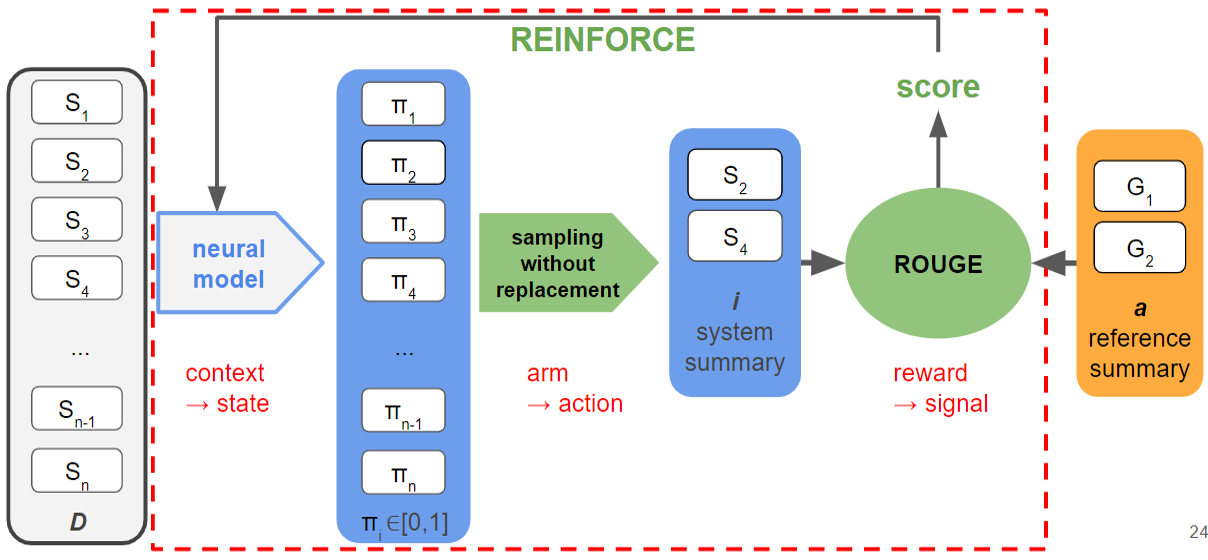
\includegraphics[width=0.9\linewidth]{fig/bsum_architecture.png}
    \caption[An overview of the BanditSum model.]{An overview of the BanditSum model. Sentence affinity scores are sampled to create hypothesis summaries, which are then scored against a reference summary using ROUGE. A gradient update is then computed using REINFORCE. Figure created by Yue Dong and used with permission.}
    \label{fig:bsum_architecture}
\end{figure}

Given a document $D$ with $n$ sentences, the neural model produces sentence affinity scores $\pi_\theta = \{ \pi_1,\dots,\pi_n \}$, where $\pi_i \in [0, 1]$.
After first using GloVe \parencite{we2_pennington2014glove} to embed each word, a word-level LSTM captures interword dependencies. In each sentence, these word representations are averaged and then passed to a sentence-level LSTM to create sentence features $h_1,\dots,h_n$. Finally, a multi-layer perceptron decoder maps $h_1,\dots,h_n$ to the sentence affinity scores $\pi_\theta = \{\pi_1,\dots,\pi_n \}$.

% Reinforcement Learning-based Objective
Using the sentence affinity scores, BanditSum now computes a gradient update following the REINFORCE algorithm \parencite{williams1992simple}. In particular, hypothesis summaries are repeatedly sampled according to $\pi_\theta$, consisting of $K$ sentences each\footnote{The authors use $K = 3$ following the average reference summary sentence length.}. Each hypothesis summary is then scored against the reference summary using a reward function based on ROUGE:

\begin{equation}
    \mathrm{R}(\mathcal{S}, \mathcal{R}_D) = \frac{1}{3}\left( \rougeone(\mathcal{S}, \mathcal{R}_D) + \rougetwo(\mathcal{S}, \mathcal{R}_D) + \rougel(\mathcal{S}, \mathcal{R}_D) \right)
\end{equation}

where $\mathcal{S}$ is the system summary and $\mathcal{R}_D$ is the reference summary. Finally, using a self-critical baseline $\overline{r}$ for variance reduction \parencite{rennie2017self}, they compute the policy gradient update as follows:

\begin{equation}
    \nabla_\theta J(\theta) = \frac{1}{B} \sum_{i=1}^{B} \nabla_\theta \log p_\theta(\mathcal{S}_i \vert D)  \left[\mathrm{R}(\mathcal{S}_i, \mathcal{R}_D) - \overline{r} \right] 
\end{equation}

where $p_\theta (\mathcal{S}_i \vert D)$ is the joint probability of including the sentences in $\mathcal{S}_i$ (i.e. according to $\pi_\theta$). This equation corresponds to the update equation given by REINFORCE \cite{williams1992simple}.

\subsection{Analysis}
% D_early vs D_late experiments, non-autoregressivity
One of BanditSum's key properties is that the model is \textbf{non-autoregressive}, meaning that the decision to include sentence $s_i$ does not explicitly depend on sentences $s_1,\dots,s_{i-1}$. An example of an autoregressive model is given by SummaRuNNer \parencite{ext5_summarunner}, whose ``summary-so-far'' representation recursively depends on previous summary decisions (see Equations \ref{eq:autoregressive-1} and \ref{eq:autoregressive-2}).

\begin{figure}[t]
    \centering
    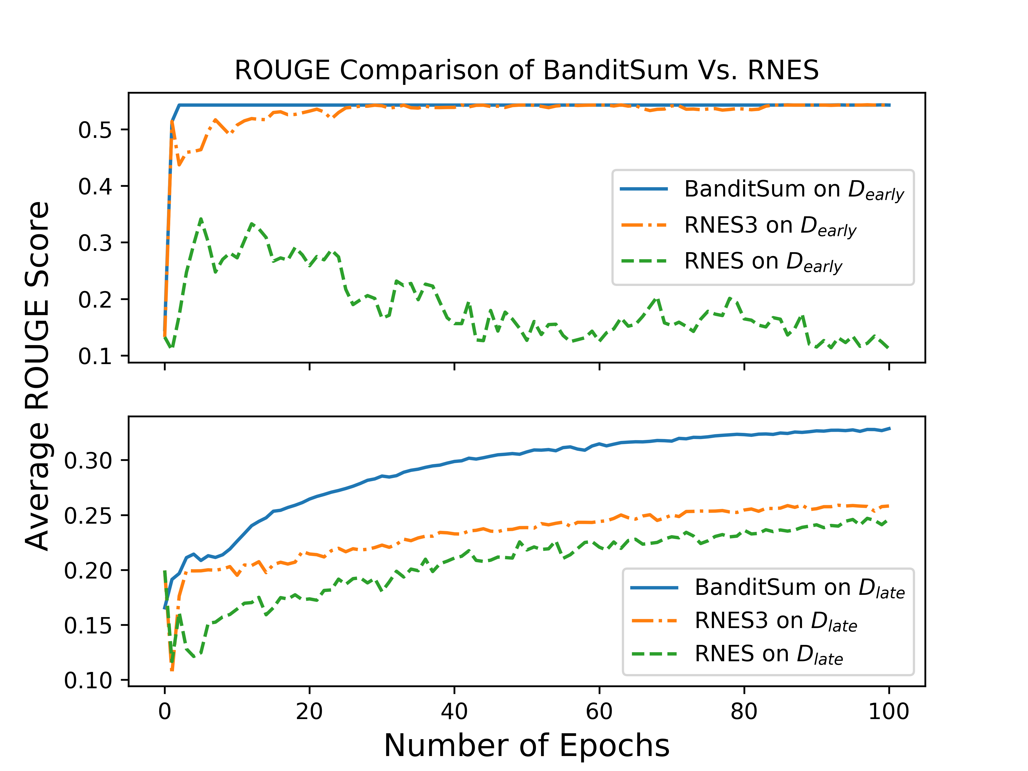
\includegraphics[width=0.8\linewidth]{fig/bsum_early_late.png}
    \caption[Comparison of BanditSum and RNES on \Dearly{} and \Dlate{} subsets.]{Comparison of BanditSum and RNES on \Dearly{} and \Dlate{} subsets. While performance is roughly similar on \Dearly{}, BanditSum dominates over RNES on \Dlate{}. Figure from \cite{dong2018banditsum}.}
    \label{fig:bsum_early_late}
\end{figure}

BanditSum's authors conjecture that autoregressive models are more likely to suffer from lead bias issues. Autoregressive models must decide whether to include early sentences before fully evaluating later sentences, and this may lead the models to erroneously include earlier sentences in their summaries. To verify this claim, the authors annotate articles from the validation set by an extractive index $\overline{idx}$, denoting whether an oracle-generated extractive summary appears earlier or later in the document. Articles are then sorted according to  $\overline{idx}$, and two datasets are created. \Dearly{} is formed from the top 50 documents w.r.t. $\overline{idx}$ (i.e. best summary appears earlier), while \Dlate{} contains the lowest-scoring 50 articles (i.e. best summary appears late). Finally, both BanditSum and an autoregressive model RNES \parencite{DBLP:conf/aaai/WuH18} are trained and evaluated on the \Dearly{} and \Dlate{} subsets. The results are displayed in Figure \ref{fig:bsum_early_late}.

% Results from this experiment
While BanditSum and RNES perform similarly on \Dearly{}, BanditSum eclipses RNES on \Dlate{}, converging much quicker to higher scoring summaries. Owing to its non-autoregressive formulation, BanditSum can produce more effective summaries when summary-worthy sentences occur later in the article. This fact provides a good basis for performing lead bias experiments with BanditSum, as we would prefer a model that is not inherently biased towards earlier occurring sentences.

\section{Lead Bias of News Systems}\label{sec:perturb}
While the observed performance drops in \cite{kedzie2018content} may be due to the destruction of position cues, they may also arise because the article's coherence and context were lost. We explore this phenomenon more deeply by distorting sentence order in a multitude of ways. 

We manipulate the CNN / Daily Mail dataset to preserve sentence position information at different levels. For each setting, we train separate instances of BanditSum, then test the model on the other datasets. In the \textbf{random} setting, sentences are shuffled randomly; in \textbf{reverse}, they are in reverse order; in \textbf{insert-lead} and \textbf{insert-lead3}, we insert an out-of-document sentence (chosen randomly from the corpus) as the first sentence or randomly as one of the first three sentences, respectively. Finally, \textbf{original} preserves the original ordering.

\begin{table}[t]
\centering
\small
\begin{tabular}{c|ccccc}
\toprule
\diagbox{Train setting}{Test setting}	&	original	&	random	&	reverse	&	insert-lead	&	insert-lead3	\\ \hline
Lead-3 baseline	&	32.68	&	22.81	&	17.94	&	27.67	&	27.68	\\ \hline
original	&	\textbf{33.85}	&	26.18	&	20.71	&	31.71	&	31.11	\\
random	&	30.88	&	\textbf{29.70}	&	29.79	&	29.97	&	30.09	\\
reverse	&	21.35	&	26.32	&	\textbf{33.59}	&	21.63	&	21.65	\\
insert-lead	&	33.21	&	26.07	&	20.70	&	\textbf{33.41}	&	31.59	\\
insert-lead3	&	32.29	&	25.57	&	20.22	&	32.92	&	\textbf{32.15}	\\ \bottomrule
\end{tabular}
\caption[BanditSum's performance on perturbed datasets]{BanditSum's performance---calculated as the average between ROUGE-1,-2, and -L F1---on the CNN/Daily Mail validation set. The sentence position information is perturbed at different levels.}
\label{tab:data_manipulation}
\end{table}

\begin{table}[t]
    \centering
    \begin{tabular}{c|c|c}
    \toprule
    Train setting	&	Average of ROUGE-1, -2, -L	&	Standard Deviation	\\ \hline
    Lead-3 baseline	&	25.76	&	5.00	\\ \hline
    original	&	28.71	&	4.72	\\
    random	&	\textbf{30.09}	&	\textbf{0.42}	\\
    reverse	&	24.91	&	4.72	\\
    insert-lead	&	29.00	&	4.93	\\
    insert-lead3	&	28.63	&	4.98	\\ \bottomrule
    \end{tabular}
    \caption[BanditSum's average performance on perturbed datasets.]{Average ROUGE-1, -2 and -L scores and standard deviation on the CNN / Daily Mail validation set using different training settings.}
    \label{tab:data_manipulation_mean}
\end{table}

In Table \ref{tab:data_manipulation} and \ref{tab:data_manipulation_mean}, we show BanditSum's performance when trained and tested on the various datasets.
All models (except random) perform worse when tested on a mismatched data perturbation. Even when the distortion is at a single lead position in \textbf{insert-lead} and \textbf{insert-lead3}, the performance on the original data is significantly lower than when trained without the distortion.

These results corroborate \cite{kedzie2018content}'s findings for RL-based systems. Similar results hold two other models we test: RNES \parencite{DBLP:conf/aaai/WuH18} drops 4.2 and Refresh \parencite{DBLP:Narayan/2018} drops 3.4 points in average ROUGE when trained on shuffled data and tested on the original dataset.

% Conclusions
The results in Table \ref{tab:data_manipulation} are worrying as the large drops between mismatched train and test settings suggest that position cues are a dominating signal for BanditSum. These findings suggest that BanditSum may largely ignore semantic content in favour of cheap positional cues. Obviously, this exploit will not work for news articles where summary-worthy content appears later. Beyond the news domain, other summarization domains may contain their own positional biases and similarly influence automatic learners. More generally, future summarization systems which attempt to create summaries across many domains cannot solely rely on positional cues if these signals change across domains. In order to be effective, systems must learn to balance between exploiting positional cues in the data and understanding the underlying semantic content.

Interestingly, the \textbf{random} model has the 
best mean performance and the lowest variation, indicating that removing or lessening position bias may allow a model to focus on learning robust sentence semantics. Following this observation, we explore novel techniques aimed at reducing the influence of lead bias on the learning process.

\section{Auxiliary Loss Objective}
Motivated by the experiments in Section \ref{sec:perturb}, we set towards designing methods to reduce models' dependence on positional cues. We observe that in general, BanditSum tends to converge to a low-entropy policy, in the sense that the model's affinity scores are either 1 or 0 at the end of training. Regularizing low-entropy policies can increase a model's propensity to explore potentially good states or stay close to a known good policy \parencite{nachum2017improving, galashov2019information}. We extend this idea to summarization by introducing a ROUGE-based loss which regularizes the model policy using an estimate of the value of individual sentences.

As the goal is to guide the model towards properly valuing sentences, we must first approximate the true value of each sentence in a document. These sentence-level estimates are computed as a categorical distribution $P_R$ over the document:
\begin{equation}
    P_R( x = i ) = \frac{r(s_i, \mathcal{G})}{\sum_{j=1}^{n}{r(s_j, \mathcal{G})}}
\end{equation}
where $r$ is the average of ROUGE-1, -2 and -L F\textsubscript{1} scores between sentence $s_i$ in the article and the reference summary $\mathcal{G}$. Since ROUGE measures lexical overlap, this distribution provides a good approximation of each sentence's relevance to the reference answer.

We would like the model's predictive distribution $P_\mathcal{M}$ to approximately match $P_R$. To compute $P_\mathcal{M}$, we normalize the model's predicted sentence scores. In other words, if the model outputs sentence affinity scores $\pi_\theta = (\pi_1,\dots,\pi_n)$, $P_\mathcal{M}$ is computed as:
\begin{equation}
    P_\mathcal{M}(x = i) = \frac{\pi_i}{\sum_{j=1}^n \pi_j}
\end{equation}

Our auxiliary loss is defined as the KL divergence: $\mathcal{L}_{\KL} = \infdiv{P_R}{P_\mathcal{M}}$. We modify the update rule using a weighted sum of the original model loss and our KL-based loss:
\begin{equation}
\label{eq:kl_loss}
    \theta^{(t+1)} = \theta^{(t)} + \alpha \left( \nabla \mathcal{L}_{\mathcal{M}}(\theta^{(t)}) + \beta \nabla \mathcal{L}_{\KL}(\theta^{(t)}) \right)
\end{equation}
Here, $\theta^{(t)}$ represents the model's parameters at time step $t$, $\mathcal{L}_{\mathcal{M}}$ is the original model's loss function, $\alpha$ is the learning rate, and $\beta$ is a hyperparameter.

Notably, $\mathcal{L}_{\KL}$ does not account for redundancy, and we do not use this measure as the sole objective function. In fact, experiments we conduct show that solely using the KL objective function does not result in improved performance.

\section{Experimental Setup}
We test our method using the CNN/Daily Mail dataset \parencite{hermann2015teaching}, building on top of the author-provided BanditSum implementation. To reduce training time, we pre-compute and store the ROUGE-1, -2, and -L average for every sentence triplet of each article, using PyTables and HDF5 \parencite{pytables, hdf5}. This allows for a considerable increase in training speed. We limit the maximum number of sentences considered in an article to the first 100. All the models were trained for 4 epochs. We set the auxiliary loss hyperparameters $\alpha=1e-4$ and $\beta=0.0095$ in Equation \ref{eq:kl_loss} based on a grid search using the Tune library \parencite{tune}.

We also train a baseline entropy model by replacing $\mathcal{L}_{\KL}$ with the negated entropy of $P_\mathcal{M}$ in Equation \ref{eq:kl_loss}. This loss penalizes low entropy, helping the model explore, but it is `undirected' compared to our proposed method. In contrast, the $\mathcal{L}_{\KL}$ loss provides an indication of each sentence's value, and is `directed' in this sense. We present the results of Lead-3 baseline (first 3 sentences), and two other competitive models -- Refresh and NeuSum \parencite{DBLP:Narayan/2018, neusum}. Lastly, we include results from an oracle summarizer, computed as the triplet of source sentences with the highest average of ROUGE-1, -2 and -L scores against the abstractive gold standard.

\section{Results}
\label{sec:result}
\begin{table}[t]
    \centering
    \small
    \begin{tabular}{l|ccc|c}
        \toprule						
        Model	&	\multicolumn{3}{c}{ROUGE}	& Lead Overlap	\\
        	&	1	&	2	&	L	&	\%	\\ \hline
        Lead-3	&	40.06	&	17.53	&	36.18	&   100.0	\\
        Oracle	&	56.53	&	32.65	&	53.12	&	27.24	\\
        Refresh	&	40.0	&	18.2	&	36.6	&	--	\\
        NeuSum	&	40.15	&	17.80	&	36.63	&	58.24	\\
        RNES	&	41.15	&	18.81	&	37.75	&	68.44	\\\hline 
        BanditSum	    &	41.68	&	18.78	&	38.00	&	69.87	\\
        B.Sum+pretrain  &   41.68   &   18.79   &   37.99   &   70.77   \\
        B.Sum+entropy	&	41.71	&	18.87	&	38.04	&	64.83	\\
        BanditSum+KL	&	\textbf{41.81*}	&	\textbf{18.96*}	&	\textbf{38.16*}	&	65.13	\\
        \bottomrule
    \end{tabular}
    \caption[Main results from auxiliary loss method on the CNN / Dailymail dataset.]{ROUGE scores for systems. Lead overlap denotes the model's overlap in extraction choices with the lead-3 baseline. Scores significantly higher than BanditSum with $p<0.001$ (bootstrap resampling test) are marked with *. Note that we are unable to evaluate Refresh on the lead overlap measure due to lack of access to the model outputs.}
    \label{tab:results}
\end{table}

Table \ref{tab:results} reports the F1 scores for ROUGE-1,-2 and -L \parencite{eva1_lin:2004:ACLsummarization}. We use the pyrouge\footnote{\url{www.github.com/bheinzerling/pyrouge}} wrapper library to evaluate the final models, while training with a faster Python-only implementation\footnote{\url{www.github.com/Diego999/py-rouge}}. We test for significance between the baseline models and our proposed techniques using the bootstrap method. This method was first recommended for testing significance in ROUGE scores in the original ROUGE paper \parencite{eva1_lin:2004:ACLsummarization}, and has subsequently been advocated as an appropriate measure in works such as \cite{dror-hitchhikers} and \cite{berg-kirkpatrick}.

The simple entropy regularizer has a small but insignificant improvement, indicating that while boosting exploration is helpful, it is too simple to provide real performance gains. In contrast, the BanditSum+KL method significantly improves over BanditSum, with an extra 0.15 ROUGE points on average. The last column reports the percentage of summary sentences which overlap with the lead. The auxiliary loss leads to a 4.7\% absolute decrease in such selections compared to the base system, while also reaching a better ROUGE score. Figure \ref{fig:train_curves} shows that the reward for the auxiliary loss model is consistently above the base.

\begin{figure}
    \centering
    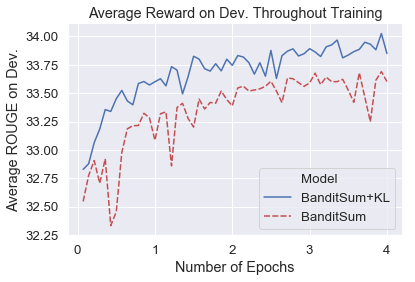
\includegraphics[width=0.75\linewidth]{fig/final_dev_fig.png}
    \caption[Training curves for BanditSum-based models.]{Training curves for BanditSum-based models. Average ROUGE is the average of ROUGE-1, -2 and -L F1.}
    \label{fig:train_curves}
\end{figure}

\section{Analysis}
Given that our method is designed to alleviate overfitting to positional cues, we suspect that the BanditSum+KL model achieves greater gains when the lead constitutes a poor summary. To test this idea, we examine the auxiliary loss model on documents where the summary is mostly comprised of lead sentences \Dearly{}, mostly sentences much later in the article \Dlate{}, and a dataset at the midway point, \Dmedian{}. To create these sets, we compute an extractive index $\overline{idx}$ for each test set document, similar to \cite{dong2018banditsum}. Given a document, we use the oracle summarizer's extracted indices $(i, j, k)$ and compute $\overline{idx}$ as:
\begin{equation}
    \overline{idx} = \frac{i + j + k}{3n}
\end{equation}
where $n$ is the number of sentences in the document.

After the test articles are ranked using the $\overline{idx}$ metric, the 100 test articles with lowest average index are \Dearly{}, the 100 with highest value are \Dlate{} and the 100 closest to the median are \Dmedian{}. In Table \ref{d_early}, we can see that the auxiliary loss model's improvements are even more amplified on \Dmedian{} and \Dlate{}. 

The second line in Table \ref{d_early} reports the oracle ROUGE scores of the best possible extractive summary. While all systems are quite close to the oracle on \Dearly{} they only reach half the performance on \Dlate{}. This gap indicates that our improvements only scratch the surface, but also that this problem is worthy and challenging to explore. 

In Figure \ref{fig:avg_pos}, we compare BanditSum and BanditSum+KL's average affinity scores. The BanditSum+KL method sharply reduces the average affinity score on the first two sentence positions, while increasing the average affinity for sentence positions 3 and beyond. This indicates that our method can help the model reach sentences further down the document. We notice similar trends for the average position selection, though the BanditSum+KL method remains far from the oracle summarizer.

We also compare model prediction distributions on an example article from the validation set in Figure \ref{fig:pred_dist}. While the BanditSum predictions forms a very low-entropy distribution, the KL loss helps even out the predictions and reach sentences further in the document.

It is worth noting that we have attempted to build a single model which can summarize both lead-biased articles and those whose information is spread throughout. Our aim was to encourage the model to explore useful regions as a way of learning better document semantics. But we hypothesize that our models can be further improved by learning to automatically predict when the lead paragraph suffices as a summary, and when the model should look further in the document.

\begin{table}
\centering
\small
\begin{tabular}{l|l|l|l}
\toprule
Model	&	$D_{\mathrm{early}}$	& $D_{\mathrm{med}}$ &	$D_{\mathrm{late}}$	\\ \hline
Lead-3	&	46.17	&	30.90	&	20.18	\\
Oracle	&	50.52	&	47.92	&	42.21	\\
NeuSum	&	40.70	&	31.26	&	20.44	\\
RNES	&	41.76   &   32.11   &   20.62	\\ \hline
BanditSum	&	43.10	&	32.65	&	21.63	\\
BanditSum+entropy	&	41.96	&	32.59	&	22.12	\\
BanditSum+KL	&	42.63	&	33.05	&	21.96	\\
\bottomrule
\end{tabular}
\caption[ROUGE scores on $D_{\mathrm{early}}$, $D_{\mathrm{med}}$ and $D_{\mathrm{late}}$ subsets.]{Average ROUGE-1, -2 and -L F1 scores on $D_{\mathrm{early}}$, $D_{\mathrm{med}}$ and $D_{\mathrm{late}}$ subsets. Each set contains 100 documents.}
\label{d_early}
\end{table}

\begin{figure}[h]
\centering
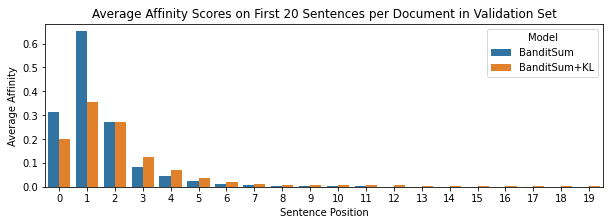
\includegraphics[width=0.9\linewidth]{fig/avg_affs.png}
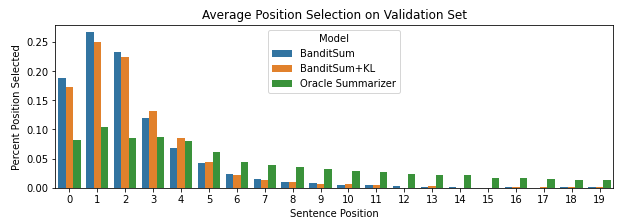
\includegraphics[width=0.9\linewidth]{fig/pos_avg.png}
\caption[Average affinity scores and average position selected for the BanditSum and BanditSum+KL models.]{(Top) Average affinity scores for the BanditSum and BanditSum+KL models. Note that the original model has far higher affinity on average for the first two sentence positions, while our proposed model has a more even distribution. (Bottom) Average position selected for the same models. We observe similar trends as the affinity score distribution, though the BanditSum+KL method remains far from the oracle positions.}
\label{fig:avg_pos}
\end{figure}

\begin{figure}[h]
    \centering
    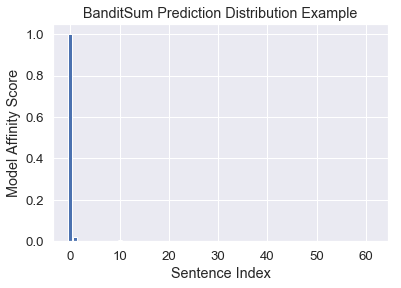
\includegraphics[width=0.48\textwidth]{fig/banditsum_pred_dist.png}
    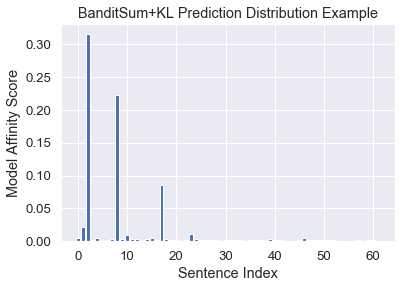
\includegraphics[width=0.48\textwidth]{fig/mixed_rouge_pred_dist.png}
    \caption[Example of the BanditSum vs. BanditSum+KL prediction distributions.]{Example of the BanditSum prediction distribution (left) vs. the BanditSum+KL prediction distribution (right) on the same given article from the validation set. The original formulation is more prone to lead bias compared to our proposed method, as demonstrated here.}
    \label{fig:pred_dist}
\end{figure}